% Compilar a .pdf con LaTeX (pdflatex)
% Es necesario instalar Beamer (paquete latex-beamer en Debian)
%


\documentclass{beamer}
\usetheme{Warsaw}
\useoutertheme{infolines}
%\usebackgroundtemplate{
\includegraphics[width=\paperwidth]{format/libresoft-bg-soft.png}}
\usepackage[spanish]{babel}
\usepackage[utf8]{inputenc}
\usepackage{graphics}
\usepackage{amssymb} % Simbolos matematicos

%\definecolor{libresoftgreen}{RGB}{162,190,43}
%\definecolor{libresoftblue}{RGB}{0,98,143}

%\setbeamercolor{titlelike}{bg=libresoftgreen}

%% Metadatos del PDF.
\hypersetup{
  pdftitle={Frikiminutos 2015 (enero--abril)},
  pdfauthor={Jesús M. González Barahona, Gregorio Robles},
  pdfcreator={GSyC, Universidad Rey Juan Carlos},
  pdfproducer=PDFLaTeX,
  pdfsubject={},
}
%%

%%%%%%%%%%%%%%%%%%%%%%%%%%%%%%%%%%%%%%%%%%%%%%%%%%%%%%%%%%%%%%%%
%%%%%%%%%%%%%%%%%%%%%%%%%%%%%%%%%%%%%%%%%%%%%%%%%%%%%%%%%%%%%%%%
% include-only                                                 %
%%%%%%%%%%%%%%%%%%%%%%%%%%%%%%%%%%%%%%%%%%%%%%%%%%%%%%%%%%%%%%%%
%%%%%%%%%%%%%%%%%%%%%%%%%%%%%%%%%%%%%%%%%%%%%%%%%%%%%%%%%%%%%%%%
%\includeonly{presentacion}

\AtBeginSection[]
{
\begin{frame}<beamer>
\begin{center}
{\Huge \insertsection}
\end{center}
\end{frame}
}

\begin{document}

\title{Frikiminutos 2015 (enero--abril)}
\subtitle{ETSIT -- URJC}
\author{Jesús M. González Barahona, Gregorio Robles Martínez}
\institute{\url{http://gsyc.es/~jgb}~~~\url{http://gsyc.es/~grex/} \\
GSyC, Universidad Rey Juan Carlos}

%\date{Enero 2015}

\frame{
\maketitle
\begin{center}

\includegraphics[width=6cm]{../format/gsyc-urjc}
\end{center}
}


% Si el titulo o el autor se quieren acortar para los pies de página
% se pueden redefinir aquí:
%\title{Titulo corto}
%\author{Autores abreviado}


%% LICENCIA DE REDISTRIBUCION DE LAS TRANSPAS
\frame{
~
\vspace{3cm}

\begin{flushright}
\copyright 2015 Gregorio Robles, Jesús M. González Barahona. \\

Algunos derechos reservados. Este artículo se distribuye bajo
la licencia ``Reconocimiento-CompartirIgual 3.0 España'' de Creative Commons,
disponible en \\
{\small \url{http://creativecommons.org/licenses/by-sa/3.0/es/deed.es}}

Este documento (o uno muy similar) está disponible en \\
\url{http://cursosweb.github.io} \\
\end{flushright}
}
%%

\frame{
\tableofcontents
}

%%%%%%%%%%%%%%%%%%%%%%%%%%%%%%%%%%%%%%%%%%%%%%%%%%%%%%%%%%%%%%%%
%%%%%%%%%%%%%%%%%%%%%%%%%%%%%%%%%%%%%%%%%%%%%%%%%%%%%%%%%%%%%%%%
% lista de temas                                               %
%%%%%%%%%%%%%%%%%%%%%%%%%%%%%%%%%%%%%%%%%%%%%%%%%%%%%%%%%%%%%%%%
%%%%%%%%%%%%%%%%%%%%%%%%%%%%%%%%%%%%%%%%%%%%%%%%%%%%%%%%%%%%%%%%
%
%

%%-----------------------------------------------------
%%-----------------------------------------------------
\section{Localizando a quien se deje}

%%-----------------------------------------------------
\begin{frame}
\frametitle{Escenario}

{\Large
Queremos saber quien está en nuestro edificio:

\begin{itemize}
\item Con el mínimo esfuerzo nuestro posible.
\item Con el mínimo esfuerzo por parte de quienes están en el edificio.
\itme Pero podemos suponer una colaboración por su parte \\
(están interesados en que se sepa que están).
\item El edificio no es muy grande, y está aislado.
\item Una solución aproximada es suficiente.
\end{itemize}
}

{\huge
\begin{center}
¿Ideas?
\end{center}
}
\end{frame}

%%-----------------------------------------------------
\begin{frame}
\frametitle{¿Y si usamos WiFi?}

{\Large
\begin{itemize}
\item Casi todos llevan teléfono
\item Casi todos llevan WiFi activado
\item Cada teléfono usa una MAC WiFi distinta
\item Podemos pedir un registro de MACs (app web simple)
\end{itemize}
}

\vspace{1cm}

{\huge
\begin{center}
¿Cómo sabemos quién está en el edificio?
\end{center}
}

\end{frame}

%%-----------------------------------------------------
\begin{frame}
\frametitle{Detectando MACs en nuestra red WiFi}

{\Large

\begin{itemize}
\item Si somos el punto de acceso (AP), sabemos todas las MAC conectadas
\item Si escuchamos en un canal, recibimos todas las MAC que emiten
\item Pero la electrónica y el software tienen que permitirlo
\end{itemize}
}

El caso de Android:

\begin{itemize}
\item Si tenemos acceso root (eg, CyanogenMod), tenemos un kernel Linux.
\item La electrónica y el software permiten modo AP.
\item Podemos ver todo lo que ve el kernel
\item De hecho, para muchas cosas no hace falta estar en modo AP.
\end{itemize}

\begin{flushright}
{\small
  \url{https://github.com/rorist/android-network-discovery}
}
\end{flushright}
\end{frame}

%
%

%%-----------------------------------------------------
%%-----------------------------------------------------
\section{¿Cómo sabe mi navegador dónde estoy?}

%%-----------------------------------------------------
\begin{frame}
\frametitle{Pero qué listo es tu móvil}

{\Large
Vete a un sitio donde no haya cobertura GPS

\begin{flushright}
o deshabilita el GPS de tu móvil
\end{flushright}

Lanza la aplicación Google Maps

\begin{flushright}
O busca tu localización en OpenStreetMap

\url{http://www.openstreetmap.org}
\end{flushright}
}

{\huge
\begin{center}
¿Cómo es posible?
\end{center}
}
\end{frame}

%%-----------------------------------------------------
\begin{frame}
\frametitle{Servicios de localización}

{\Large
Bases de datos con coordenadas de puntos de medida de:

\begin{itemize}
\item potencia recibida de puntos de acceso WiFi (MAC, SSID)
\item potencia recibida de estaciones base de redes móviles (CellID)
\end{itemize}

También pueden incluir geolocalización de direcciones IP

\begin{flushright}
\url{http://en.wikipedia.org/wiki/Wi-Fi_positioning_system}
\end{flushright}
}

\end{frame}


%%-----------------------------------------------------
\begin{frame}
\frametitle{Uso de servicios de localización}

{\Large
Ejemplo: Google Play Location Services \\
}
\begin{flushright}
\url{https://developer.android.com/google/play-services/location.html}
\end{flushright}

{\Large
Ejemplo: API JavaScript de Firefox \\
}

\begin{flushright}
\url{https://www.mozilla.org/en-US/firefox/geolocation/} \\
\url{https://developer.mozilla.org/en-US/docs/Web/API/Geolocation/Using_geolocation}
\end{flushright}
\end{frame}

%%-----------------------------------------------------
\begin{frame}
\frametitle{Mozilla Location Service y Stumbler}

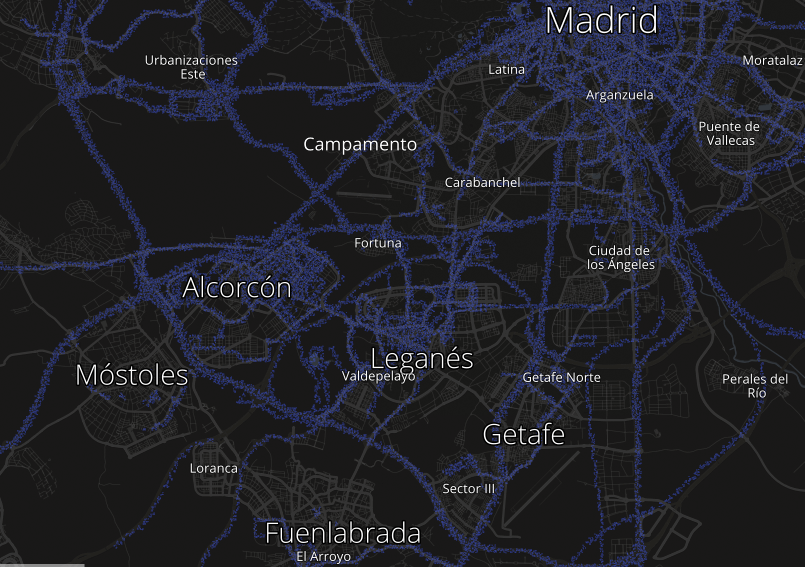
\includegraphics[height=6cm]{figs/mozilla-location-map}

\begin{flushright}
  \url{https://location.services.mozilla.com/map} \\
  \url{https://location.services.mozilla.com/} \\
\end{flushright}
\end{frame}

%%-----------------------------------------------------
\begin{frame}
\frametitle{OpenCellID}

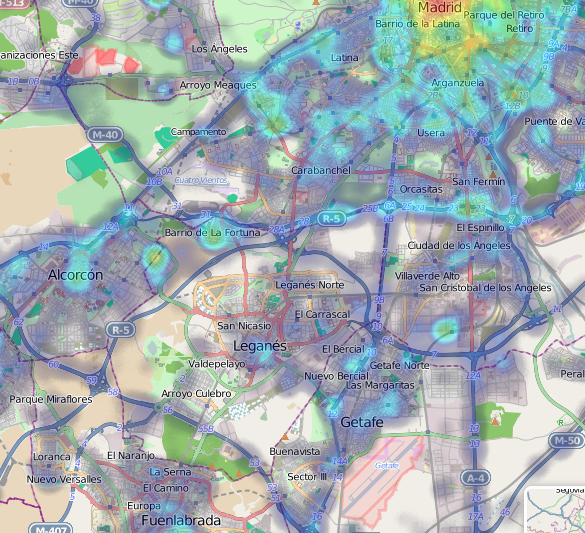
\includegraphics[height=6cm]{figs/opencellid-map}

\begin{flushright}
  \url{http://opencellid.org/} \\
  \url{http://wiki.opencellid.org/wiki/What_is_OpenCellID} \\
  \url{http://wiki.opencellid.org/wiki/Data_sources} \\
\end{flushright}
\end{frame}

%
%

%%-----------------------------------------------------
%%-----------------------------------------------------
\section{La maravillosa Wayback Machine}

%%-----------------------------------------------------
\begin{frame}
\frametitle{¿Cómo era la web de la URJC?}


\includegraphics[height=6cm]{figs/web-urjc-2014}

{\Large
\begin{flushright}
2014
\end{flushright}
}
\end{frame}

%%-----------------------------------------------------
\begin{frame}
\frametitle{¿Cómo era la web de la URJC?}


\includegraphics[height=6cm]{figs/web-urjc-2011}

{\Large
\begin{flushright}
2011
\end{flushright}
}
\end{frame}

%%-----------------------------------------------------
\begin{frame}
\frametitle{¿Cómo era la web de la URJC?}

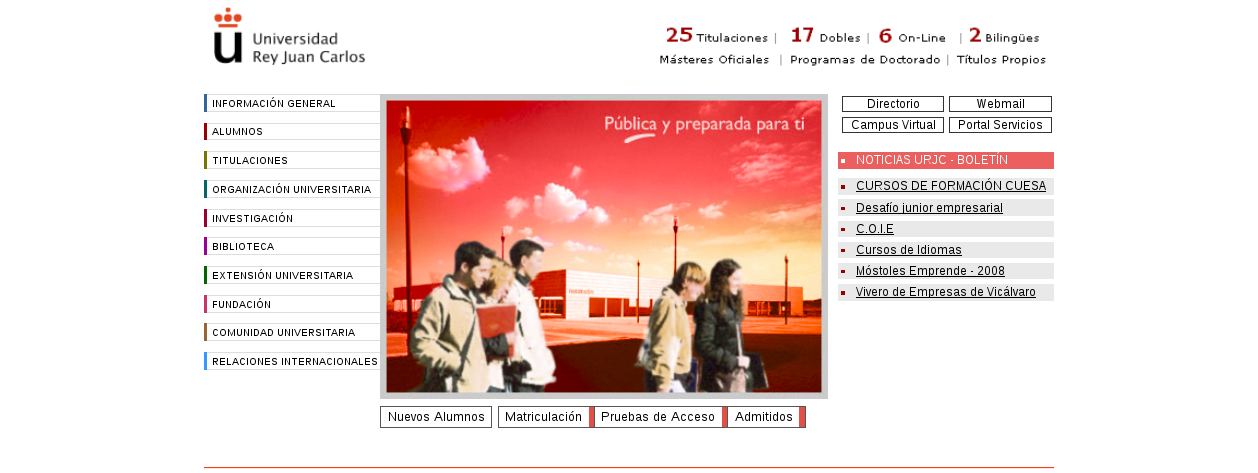
\includegraphics[height=6cm]{figs/web-urjc-2008}

{\Large
\begin{flushright}
2008
\end{flushright}
}
\end{frame}

%%-----------------------------------------------------
\begin{frame}
\frametitle{¿Cómo era la web de la URJC?}

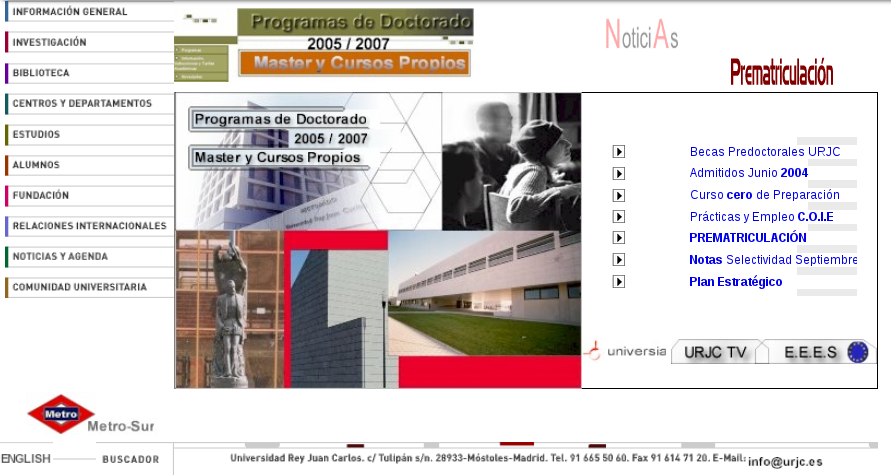
\includegraphics[height=6cm]{figs/web-urjc-2004}

{\Large
\begin{flushright}
2004
\end{flushright}
}
\end{frame}

%%-----------------------------------------------------
\begin{frame}
\frametitle{Bienvenidos a la maravillosa Wayback Machine}

{\Large
\begin{itemize}
\item Copias sitios web en distintos momentos del pasado
\item Parte del Internet Archive
\item Proporiciona una interfaz web...
\item ...y una API
\end{itemize}

\begin{flushright}
\url{https://archive.org/web/} \\
\url{https://archive.org/help/wayback_api.php} \\
\end{flushright}
}


\end{frame}





\end{document}
